\textbf{\large Задача №3}\\
\hspace*{0.5cm}Построить график функции $F(t) = \int\limits_{-1}^0 x^2 |x-t|\,dx$.\\[0.5cm]
\textbf{Решение:}\\
\hspace*{0.5cm}
Рассмотрим 3 случая
\begin{enumerate}
	\item $t \leqslant -1$, тогда
	\[F(t) = \int_{-1}^0 x^2(x-t)\, dx = \int_{-1}^0 (x^3 - x^2t)\,dx = \left.\left(\frac{x^4}{4} - \frac{x^3t}{3} \right)\right|_{x=-1}^{x=0} = -\frac14-\frac t3\]
	
	\item $-1<t<0$, тогда
	\[\begin{aligned}
		&F(t) = \int_{-1}^tx^2(t-x)\,dx + \int_t^0 x^2 (x-t) \,dx = \int_{-1}^t(x^2t-x^3)\,dx + \int_t^0(x^3-x^2t)\,dx = {}\\
		{}&= \left.\left(\frac{x^3t}{3} - \frac{x^4}{4} \right)\right|_{x=-1}^{x=t} + \left.\left(\frac{x^4}{4} - \frac{x^3t}{3} \right)\right|_{x=t}^{x=0} = \frac{t^4}{3}-\frac{t^4}{4} - \left(-\frac t3 - \frac14\right) + 0 - \left(\frac{t^4}{4} - \frac{t^4}{3}\right) = \frac{t^4}{6} + \frac{t}{3} + \frac{1}{4}
	\end{aligned}\]
	
	\item $t \geqslant 0$, тогда
	\[F(t) = \int_{-1}^0 x^2(t-x)\, dx = \int_{-1}^0 (x^2t - x^3)\,dx = \left.\left(\frac{x^3t}{3} - \frac{x^4}{4} \right)\right|_{x=-1}^{x=0} = \frac t3 + \frac14\]
\end{enumerate}

Таким образом
\[F(t) = \begin{cases}\displaystyle
	-\frac13 t - \frac14, &\text{при } t \leqslant -1 \\[8pt]
	\displaystyle \frac16 t^4 + \frac13 t + \frac14, &\text{при } -1< t < 0 \\[8pt]
	\displaystyle \frac13 t + \frac14, &\text{при } t \geqslant 0
\end{cases}\]
Можно вычислить, что  $a = F(-1) = \frac{1}{12}$, $b = F(0) = \frac14$.
Найдём точку минимума функции $g(t) = \frac16 t^4 + \frac13 t + \frac14$:
$g'(t) = \frac23t^3 + \frac13 = \frac13 (2t^3 + 1)$; $g'(t) = 0 \Leftrightarrow t = -\frac{1}{\sqrt[3]{2}}$.
И $m = F\left(-\frac{1}{\sqrt[3]{2}}\right) = \frac{1}{12}\cdot\left(2^{-\frac13} - 2^{\frac53}+3\right)$.
Поэтому график функции $F$ выглядит так:
\begin{center}
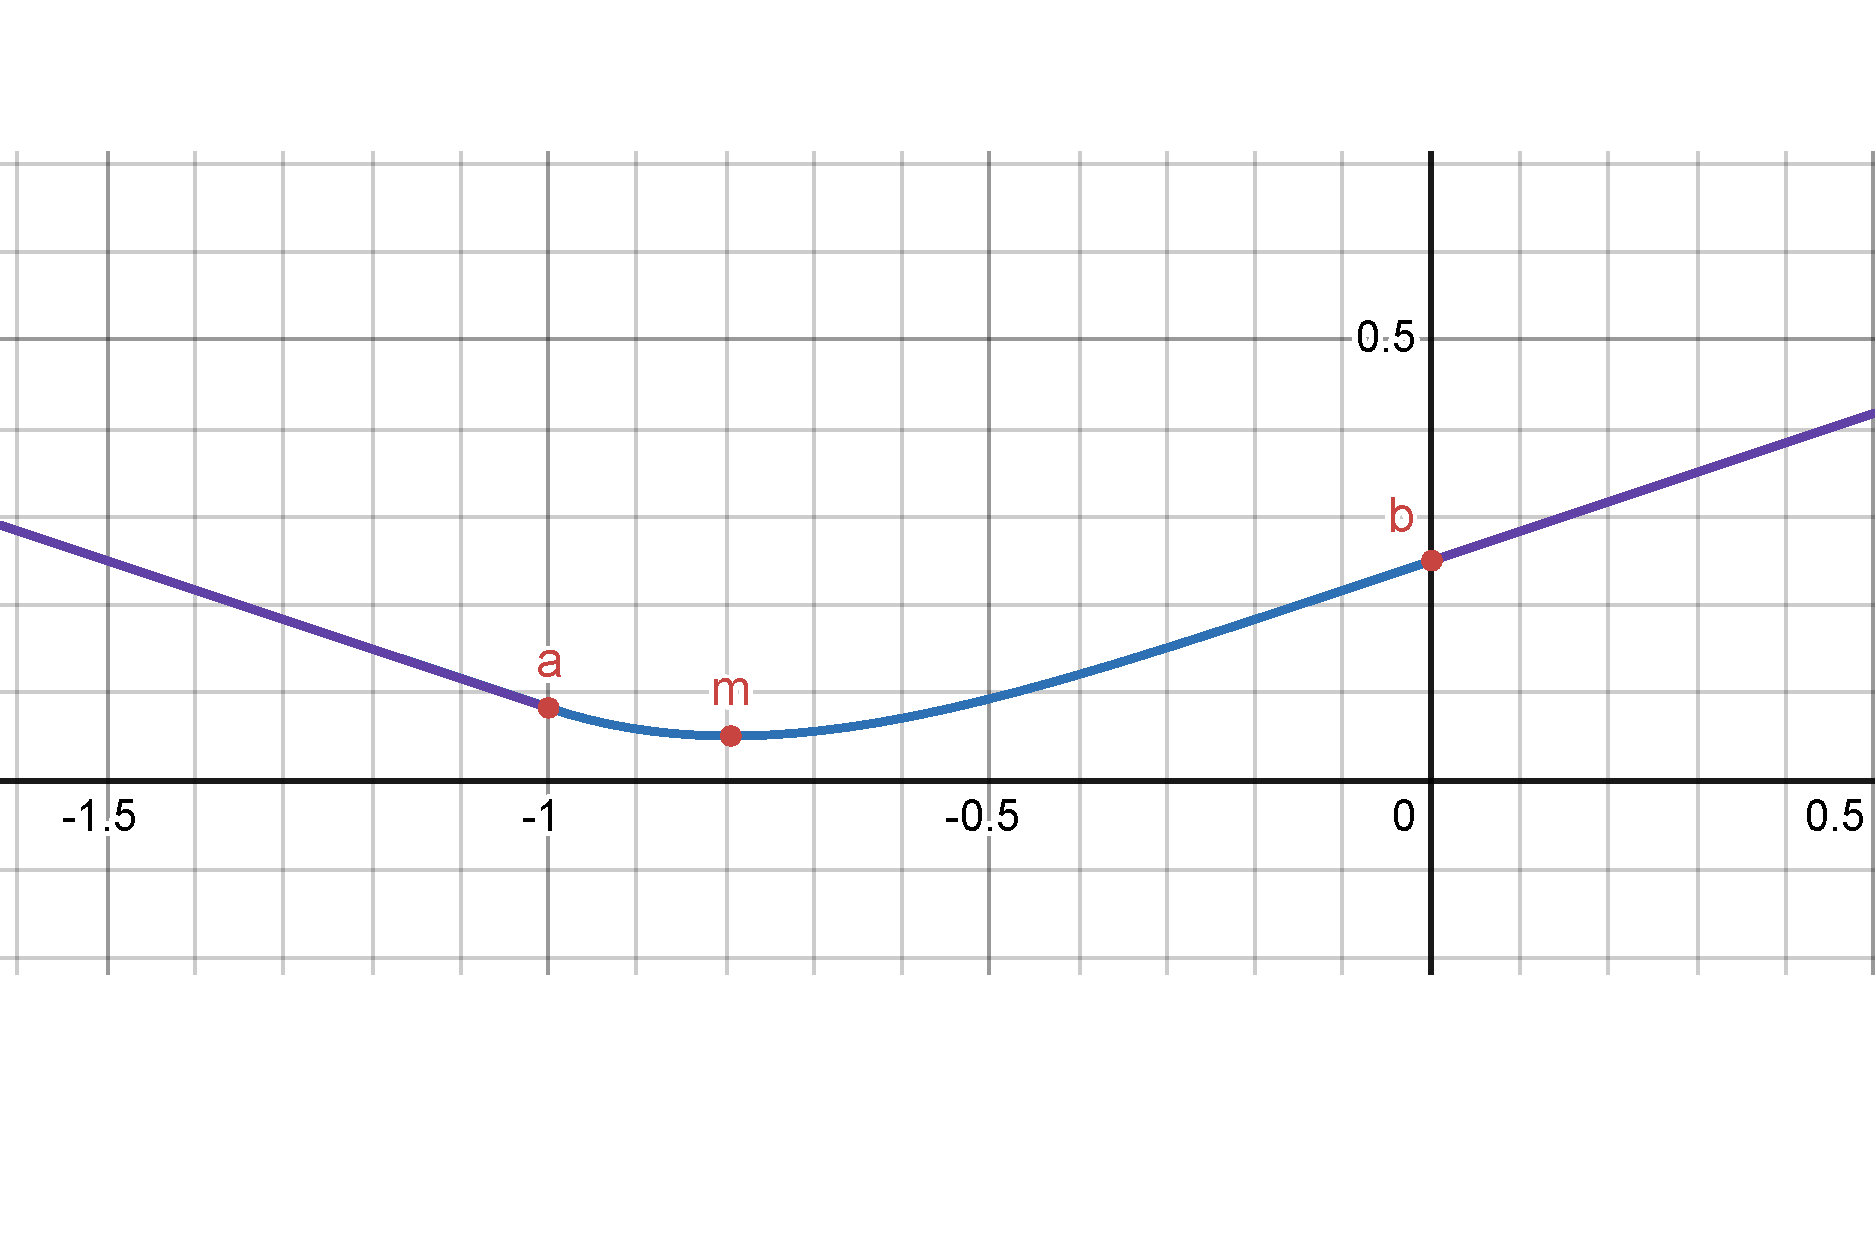
\includegraphics[width=\textwidth]{graphic.pdf}
\end{center}